\documentclass{standalone}
\usepackage{pgf-umlcd}

\renewcommand{\unidirectionalAssociation}[4]
{
  \draw[umlcd style, ->] (#1) -- (#4)
  node[near end, auto]{#2}
  node[near end, auto,swap]{#3};
}

\begin{document}
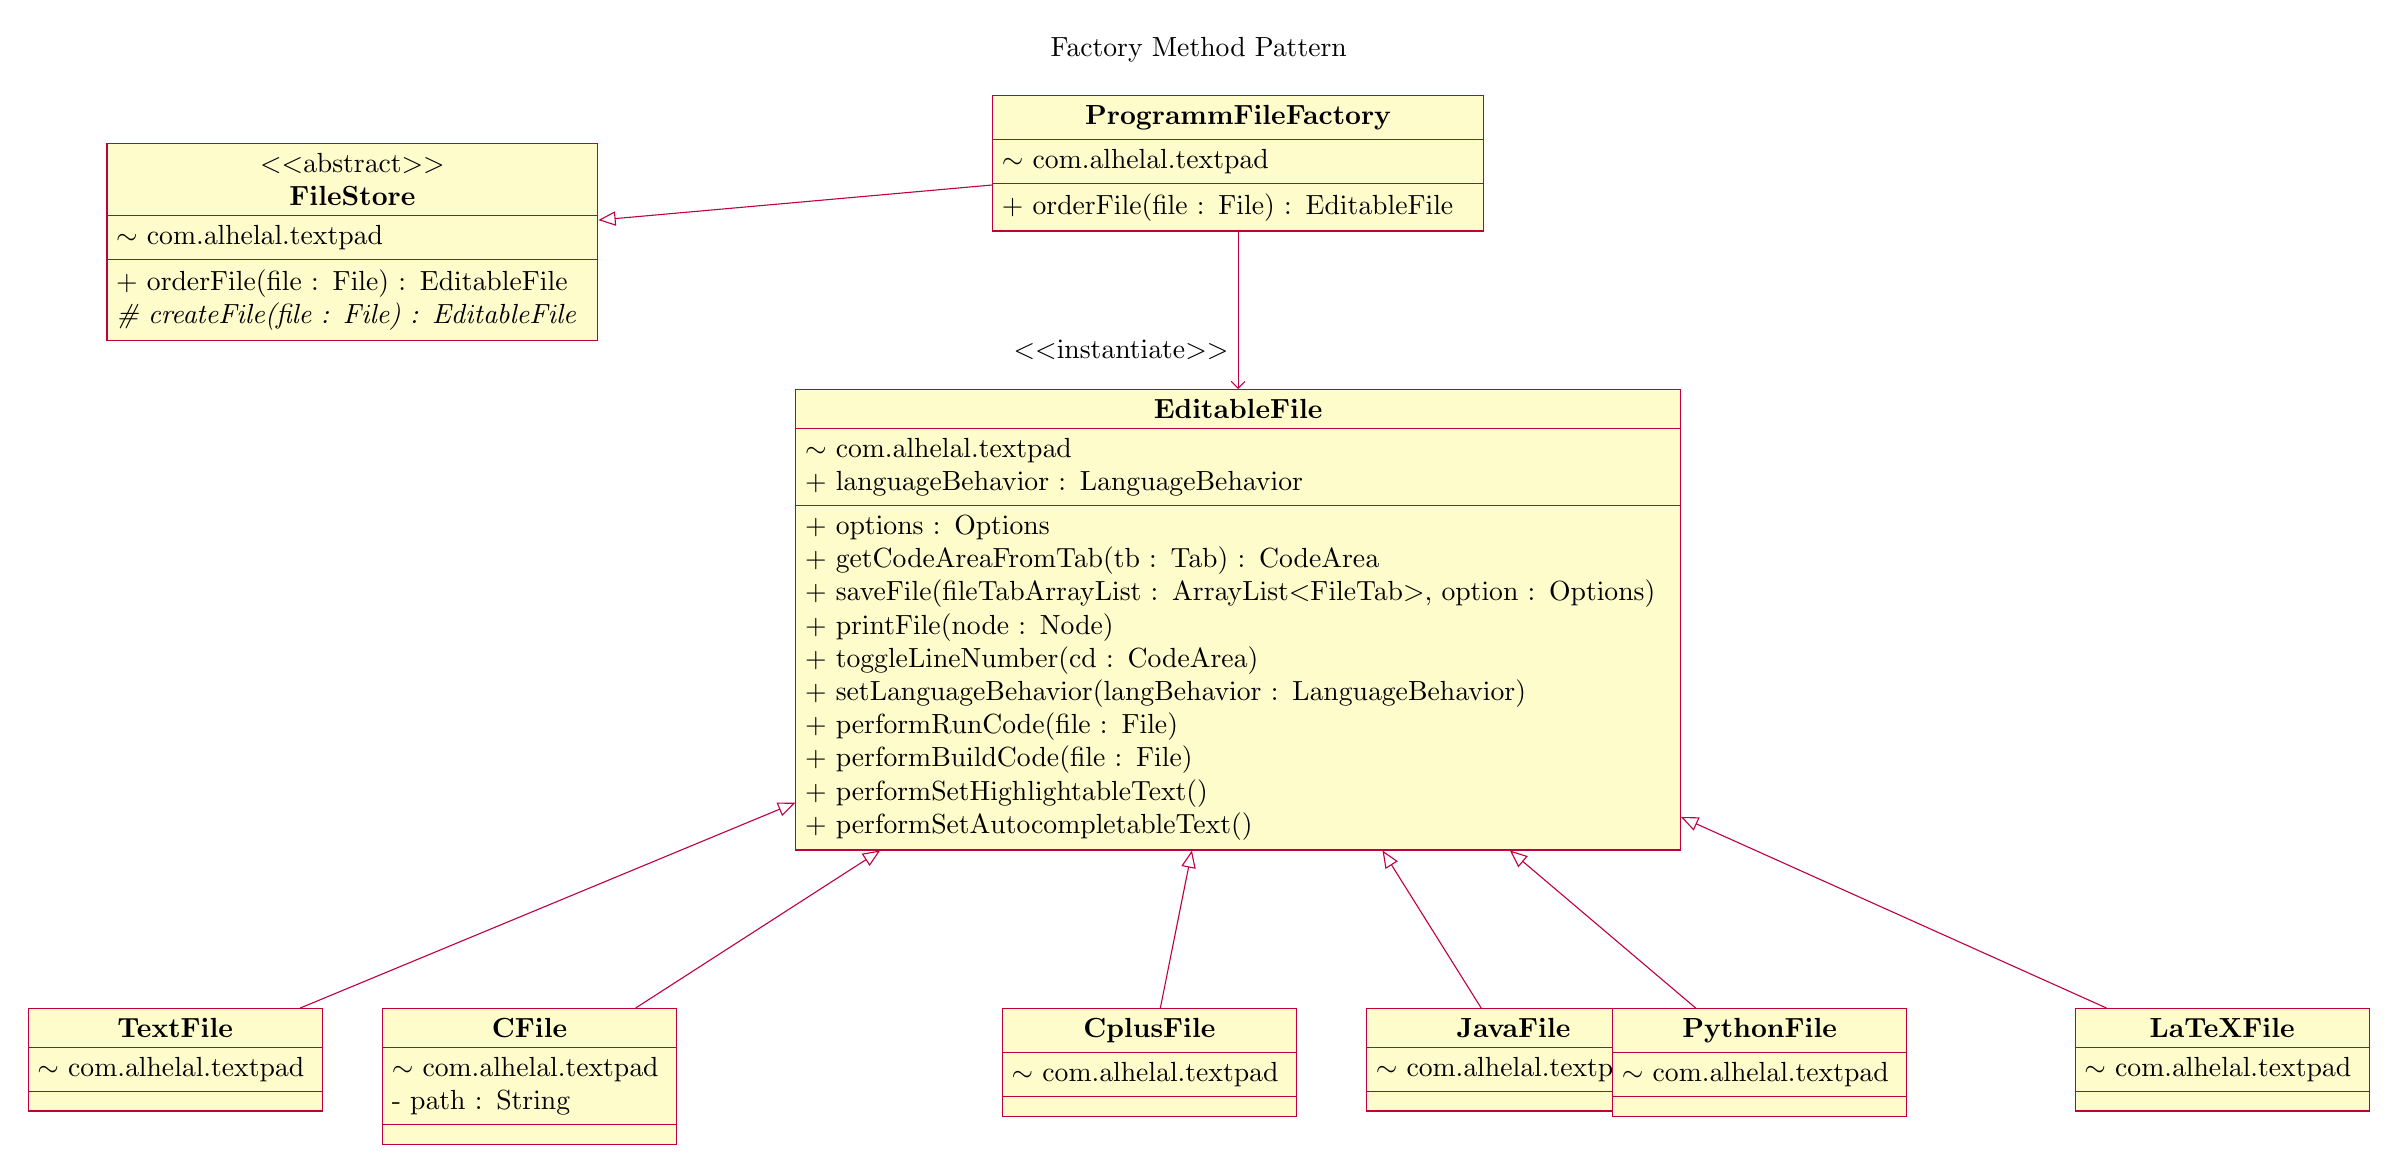
\begin{tikzpicture}

  \begin{abstractclass}[text width = 6cm]{FileStore}{0,0}
    \attribute{$\sim$ com.alhelal.textpad}
    \operation{+ orderFile(file : File) : EditableFile} 
    \operation[0]{\# createFile(file : File) : EditableFile}
  \end{abstractclass}

  \begin{class}[text width = 6cm,anchor = west,xshift = 5cm,yshift = 1cm]{ProgrammFileFactory}{FileStore.east}
    \inherit{FileStore}
    \attribute{$\sim$ com.alhelal.textpad}
    \operation{+ orderFile(file : File) : EditableFile} 
  \end{class}

  \begin{class}[text width = 11cm, yshift = -2cm]{EditableFile}{ProgrammFileFactory.south}
    \attribute{$\sim$ com.alhelal.textpad}
    \attribute{+ languageBehavior : LanguageBehavior} 
    \operation{+ options : Options} 
    \operation{+ getCodeAreaFromTab(tb : Tab) : CodeArea} 
    \operation{+ saveFile(fileTabArrayList : ArrayList$<$FileTab$>$, option : Options)}
    \operation{+ printFile(node : Node)}
    \operation{+ toggleLineNumber(cd : CodeArea)}
    \operation{+ setLanguageBehavior(langBehavior : LanguageBehavior)}
    \operation{+ performRunCode(file : File)}
    \operation{+ performBuildCode(file : File)}
    \operation{+ performSetHighlightableText()}
    \operation{+ performSetAutocompletableText()}
  \end{class}

  \begin{class}[text width = 3.5cm,anchor=north east,yshift = -2cm, xshift=-6cm]{TextFile}{EditableFile.south west}
    \inherit{EditableFile}
    \attribute{$\sim$ com.alhelal.textpad}
  \end{class}

  \begin{class}[text width = 3.5cm,anchor=north east,yshift = -2cm, xshift = -1.5cm]{CFile}{EditableFile.south west}
    \inherit{EditableFile}
    \attribute{$\sim$ com.alhelal.textpad}
    \attribute{- path : String}
  \end{class}

  \begin{class}[text width=3.5cm,anchor=north west,yshift = -2cm,xshift=-3cm]{CplusFile}{EditableFile.south}
    \inherit{EditableFile}
    \attribute{$\sim$ com.alhelal.textpad}
  \end{class}
  
  \begin{class}[text width  = 3.5cm, anchor = north west, yshift = -2cm, xshift = -4cm]{JavaFile}{EditableFile.south east}
    \inherit{EditableFile}
    \attribute{$\sim$ com.alhelal.textpad}
  \end{class}

  \begin{class}[text width = 3.5cm,yshift = -2cm,xshift = 1cm]{PythonFile}{EditableFile.south east}
    \inherit{EditableFile}
    \attribute{$\sim$ com.alhelal.textpad}
  \end{class}
  
  \begin{class}[text width = 3.5cm, anchor = north west, yshift =-2cm,xshift = 5cm]{LaTeXFile}{EditableFile.south east}
    \inherit{EditableFile}
    \attribute{$\sim$ com.alhelal.textpad}
  \end{class}
  \unidirectionalAssociation{ProgrammFileFactory}{}{$<<$instantiate$>>$}{EditableFile}
  \node [above=3mm] at (current bounding box.north) {Factory Method Pattern};
\end{tikzpicture}
\end{document}
